Standard tests for harmful shift cannot separate two questions: did the model
get worse, or did the population just change? When deployment and training
samples barely overlap, observations from regions where only one side has data
can drive rejection even when the target did not worsen on the common support,
the region where both samples have substantial overlap.

The HELOC credit-risk dataset illustrates this failure mode. A model trained on
lower-risk applicants (external risk estimate above 63) is deployed on
higher-risk applicants (estimate at or below 63)~\cite{Gardner_2023}. Mean
predicted default risk rises from 44\% to 81\%---a large shift that could
indicate model harm or merely context change. All three standard
modes---unweighted, source-weighted, and target-weighted---reject at the
permutation minimum $p = 0.002$. Most of each population lies outside the common
support. The doubly weighted test, which adjusts both sides, does not reject
($p = 0.376$). The original rejection was driven by context change---applicant
profiles from weak-overlap regions that produce higher predicted risk---rather
than model harm on comparable cases. One-sided corrections still reject because
each corrects only one side (Figure~\ref{fig:heloc-motivating}).

\begin{figure}[t]
	\centering
	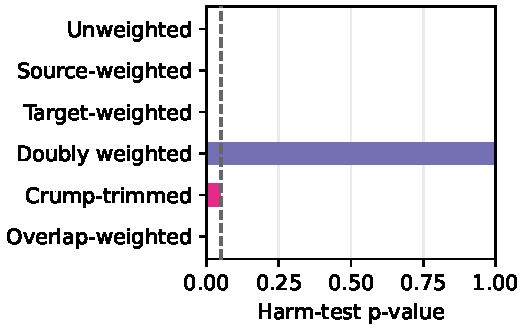
\includegraphics[width=0.92\linewidth]{figures/heloc_motivating_example_plot.pdf}
	\caption{HELOC credit-risk motivating example. Horizontal bar chart with
	weighting modes on the y-axis and harm-test $p$-value on the x-axis. The
	dashed line marks the 0.05 decision threshold. All three standard modes
	(unweighted, source-weighted, target-weighted) reject; the doubly weighted
	test does not. Effective sample sizes after reweighting to common support:
	source 401 of 1,536; target 803 of 2,776. The non-rejection indicates
	that comparable applicants receive similar predictions on common
	support.}
	\label{fig:heloc-motivating}
\end{figure}

The same ambiguity appears in the National Supported Work (NSW) employment
experiment~\cite{LaLonde_1986}, where the unweighted test fails to reject
($p = 0.350$)---a non-rejection that common-support restriction does not
reverse, illustrating that contamination can mask harm as readily as it invents
it. Together, HELOC and NSW demonstrate that weak-overlap contamination can
both invent harm and hide it.

Our starting point is D-SOS~\cite{pmlr-v180-kamulete22a}, a non-parametric
permutation test for one-sided harmful shift that compares the full observed
populations with uniform weights, allowing observations from low-overlap
regions to contaminate the comparison.\footnote{D-SOS calls the user-defined
quantity outlier scores; we use severity score to emphasize that larger
values mean worse behavior.}

We insert a weighting step that restricts the comparison to common support.
Stabilized density-ratio weights from a domain
classifier~\cite{Bickel_2007,Yamada_2013} downweight observations unlikely
to appear in the other environment---an approach the causal inference
literature developed for treatment-effect comparisons~\cite{Crump_2009,
Morgan_2015}. These weights apply to any two-sample test that accepts
per-observation weights. A single parameter $\lambda \in [0, 1]$ controls
the tradeoff between strict common-support restriction and the unweighted
comparison.

We call the resulting method CS-DSOS. The doubly weighted mode, which corrects
both source and target simultaneously, targets the common support and resolves
two-sided overlap contamination. Source-weighted and target-weighted modes serve
as asymmetric diagnostics for one-sided mismatch.

Our contributions are:
\begin{itemize}
\item CS-DSOS, a family of stabilized density-ratio weights that restrict
  harmful-shift testing to the common support. The doubly weighted mode
  corrects both source and target simultaneously and resolves two-sided
  overlap contamination, with source-weighted and target-weighted modes as
  asymmetric diagnostics for one-sided mismatch.
\item Evidence that the doubly weighted test removes false alarms from
  low-overlap contamination without attenuating power for genuine harmful
  change on the common support, across synthetic and real-world tasks.
\end{itemize}
